\documentclass[aspectratio=169]{beamer}
\usetheme{default}
\setbeamertemplate{navigation symbols}{}
\setbeamertemplate{footline}{}
\usepackage[T1]{fontenc}
\usepackage{lmodern}
\usepackage{tikz}
\usetikzlibrary{arrows.meta,positioning,fit,backgrounds}
\usepackage{xcolor}
\definecolor{navy}{HTML}{17324D}
\definecolor{blue}{HTML}{3977A8}
\definecolor{pale}{HTML}{EAF2F8}
\definecolor{teal}{HTML}{33877D}
\definecolor{gold}{HTML}{C8872F}
\definecolor{ink}{HTML}{263746}
\setbeamercolor{normal text}{fg=ink,bg=white}
\setbeamercolor{frametitle}{fg=navy,bg=white}
\setbeamerfont{frametitle}{series=\bfseries,size=\Large}
\setbeamersize{text margin left=0.48cm,text margin right=0.48cm}
\tikzset{
  block/.style={draw=blue!65!navy,fill=pale,rounded corners=2pt,align=center,
    minimum height=0.70cm,text width=1.55cm,font=\scriptsize,inner sep=3pt},
  narrow/.style={block,text width=1.30cm},
  arrow/.style={-{Stealth[length=1.7mm]},draw=blue!75!navy,line width=0.7pt},
  feedback/.style={-{Stealth[length=1.7mm]},draw=teal,line width=0.8pt},
  note/.style={font=\scriptsize,align=left,text=ink}
}
\begin{document}
\begin{frame}[t]
\frametitle{Graph of Graphs: Architecture and Current Work}
\vspace{-0.15cm}
\begin{columns}[T,onlytextwidth]
\begin{column}{0.68\textwidth}
\centering
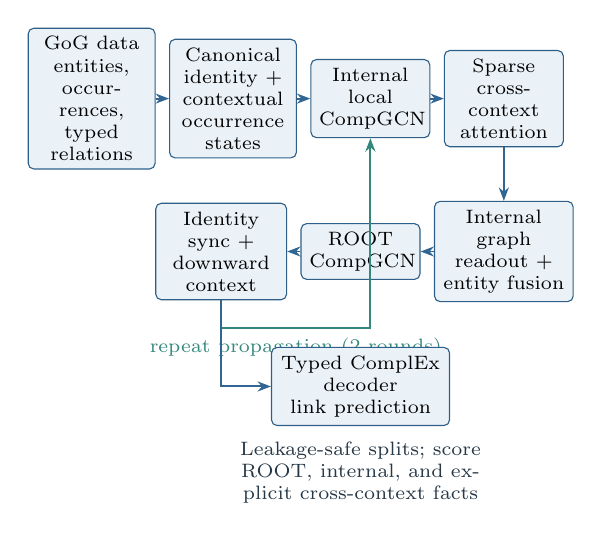
\begin{tikzpicture}[node distance=0.15cm and 0.17cm]
  \node[block,text width=1.4cm] (data) {GoG data\\entities, occurrences, typed relations};
  \node[block,text width=1.4cm,right=of data] (init) {Canonical identity +\\contextual occurrence states};
  \node[narrow,right=of init] (local) {Internal\\local\\CompGCN};
  \node[narrow,right=of local] (cross) {Sparse\\cross-context\\attention};
  \node[block,text width=1.55cm,below=0.68cm of cross] (pool) {Internal graph\\readout +\\entity fusion};
  \node[narrow,left=of pool] (root) {ROOT\\CompGCN};
  \node[block,text width=1.45cm,left=of root] (sync) {Identity sync +\\downward context};
  \draw[arrow] (data)--(init);
  \draw[arrow] (init)--(local);
  \draw[arrow] (local)--(cross);
  \draw[arrow] (cross.south)--(pool.north);
  \draw[arrow] (pool.west)--(root.east);
  \draw[arrow] (root.west)--(sync.east);
  \draw[feedback] (sync.south) -- ++(0,-0.35) -| node[pos=0.25,below,font=\scriptsize,text=teal]{repeat propagation (2 rounds)} (local.south);
  \node[block,below=0.85cm of root,text width=2.05cm,minimum height=0.62cm] (decoder)
    {Typed ComplEx decoder\\link prediction};
  \draw[arrow] (sync.south) |- (decoder.west);
  \node[below=0.08cm of decoder,note,align=center,text width=4.0cm] {Leakage-safe splits; score ROOT, internal, and explicit cross-context facts};
\end{tikzpicture}

\vspace{0.18cm}
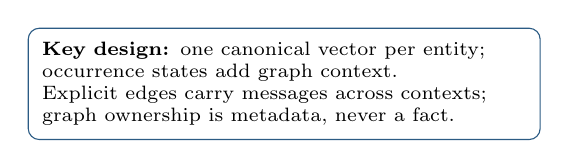
\begin{tikzpicture}[font=\scriptsize]
  \node[draw=blue!60!navy,fill=white,rounded corners,inner sep=5pt,align=left,text width=6.15cm] {
  \textbf{Key design:} one canonical vector per entity; occurrence states add graph context.\\
  Explicit edges carry messages across contexts; graph ownership is metadata, never a fact.};
\end{tikzpicture}
\end{column}

\begin{column}{0.30\textwidth}
\vspace{0.02cm}
{\color{teal}\bfseries CURRENT WORK}\par
\vspace{0.08cm}
{\small GoG encoder and typed link-prediction training pipeline implemented; currently comparing against an entity-only baseline on PrimeKG.}\par
\vspace{0.18cm}
{\color{navy}\bfseries Exploratory result}\par
\vspace{0.06cm}
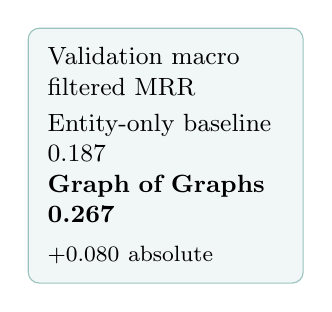
\begin{tikzpicture}
  \node[draw=teal!50,fill=teal!7,rounded corners,inner sep=7pt,align=left,text width=3.0cm,font=\small] {
    Validation macro filtered MRR\\[2pt]
    Entity-only baseline \hfill 0.187\\
    \textbf{Graph of Graphs} \hfill \textbf{0.267}\\[3pt]
    \footnotesize +0.080 absolute};
\end{tikzpicture}
\vspace{0.12cm}
{\scriptsize\color{ink}10-epoch local comparison; automatically generated split. Preliminary result, not a benchmark claim. Next: scale and validate training in Colab/GPU, then assess held-out performance.}\par
\vfill
{\tiny Source: project architecture specification and \texttt{primekg-clean-comparison} report.}
\end{column}
\end{columns}
\end{frame}
\end{document}
